\documentclass[BufferStockTheory]{subfiles}
% WARNING: AuCTeX local variables only get reset when file is loaded
% and differ between this file and BufferStockTheory.tex
% so must re-load whichever file you want to compile with C-x C-v

% WARNING: Different AucTeX execution depending on whether
% 0. Being compiled as standalone document
%    * Compile main once
%    * Then compile this one
%    * Keep compiling until nothing changes
% 0. Being compiled as subfile of main document
%    * Just compile main document repeatedly

\providecommand{\econtexRoot}{}\renewcommand{\econtexRoot}{..}
\providecommand{\econtexPaths}{}\renewcommand{\econtexPaths}{\econtexRoot/Resources/econtexPaths}
% The \commands below are required to allow sharing of the same base code via Github between TeXLive on a local machine and Overleaf (which is a proxy for "a standard distribution of LaTeX").  This is an ugly solution to the requirement that custom LaTeX packages be accessible, and that Overleaf prohibits symbolic links
\providecommand{\econtex}{\econtexRoot/Resources/texmf-local/tex/latex/econtex}
\providecommand{\econtexSetup}{\econtexRoot/Resources/texmf-local/tex/latex/econtexSetup}
\providecommand{\econtexShortcuts}{\econtexRoot/Resources/texmf-local/tex/latex/econtexShortcuts}
\providecommand{\econtexBibMake}{\econtexRoot/Resources/texmf-local/tex/latex/econtexBibMake}
\providecommand{\econtexBibStyle}{\econtexRoot/Resources/texmf-local/bibtex/bst/econtex}
\providecommand{\econtexBib}{economics}
\providecommand{\notes}{\econtexRoot/Resources/texmf-local/tex/latex/handout}
\providecommand{\handoutSetup}{\econtexRoot/Resources/texmf-local/tex/latex/handoutSetup}
\providecommand{\handoutShortcuts}{\econtexRoot/Resources/texmf-local/tex/latex/handoutShortcuts}
\providecommand{\handoutBibMake}{\econtexRoot/Resources/texmf-local/tex/latex/handoutBibMake}
\providecommand{\handoutBibStyle}{\econtexRoot/Resources/texmf-local/bibtex/bst/handout}

\providecommand{\FigDir}{\econtexRoot/Figures}
\providecommand{\CodeDir}{\econtexRoot/Code}
\providecommand{\DataDir}{\econtexRoot/Data}
\providecommand{\SlideDir}{\econtexRoot/Slides}
\providecommand{\TableDir}{\econtexRoot/Tables}
\providecommand{\ApndxDir}{\econtexRoot/Appendices}

\providecommand{\ResourcesDir}{\econtexRoot/Resources}
\providecommand{\rootFromOut}{..} % Path back to root directory from output-directory
\providecommand{\LaTeXGenerated}{\econtexRoot/LaTeX} % Put generated files in subdirectory
\providecommand{\econtexPaths}{\econtexRoot/Resources/econtexPaths}
\providecommand{\LaTeXInputs}{\econtexRoot/Resources/LaTeXInputs}
\providecommand{\LtxDir}{LaTeX/}
\providecommand{\EqDir}{Equations} % Put generated files in subdirectory


\onlyinsubfile{% https://tex.stackexchange.com/questions/463699/proper-reference-numbers-with-subfiles
    \csname @ifpackageloaded\endcsname{xr-hyper}{%
      \externaldocument{\econtexRoot/BufferStockTheory}% xr-hyper in use; optional argument for url of main.pdf for hyperlinks
    }{%
      \externaldocument{\econtexRoot/BufferStockTheory}% xr in use
    }%
    \renewcommand\labelprefix{}%
    % Initialize the counters via the labels belonging to the main document:
    \setcounter{equation}{\numexpr\getrefnumber{\labelprefix eq:Dummy}\relax}% eq:Dummy is the last number used for an equation in the main text; start counting up from there
}


\onlyinsubfile{\externaldocument{ProjectDLO}} % Get xrefs -- esp to appendix -- from main file; only works properly if main file has already been compiled;

\begin{document}

% Attempted to make all lines used for Web version contain {Web} (or version with only single curly brace at end) so can be removed with sed
\providecommand{\versn}{pdf} % Version; like, web or pdf or journal submission
\ifthenelse{\boolean{Web}}{    % {Web}
  \renewcommand{\versn}{Web}     % Too hard to figure out passing -output-directory through make4ht through htlatex, so web version is compiled with junk files in main directory
  \renewcommand{\rootFromOut}{.} % {Web}
}{}  % {Web}

% Tiny info header at top to track git commit
%\hfill{\tiny \jobname~\versn~\today~{at} \DTMcurrenttime, \input{\ResourcesDir/.git-source-commit}~~\input{\ResourcesDir/.git-public-commit}}

\title{Price Rigidities \\ An attempt at a new angle}

\author{David L. Osten\authNum}

\keywords{Price Rigidity, Inflation Expectations, Market Power, Search Cost}

%\jelclass{D81, D91, E21 \par
%  \href{https://econ-ark.org}{
\includegraphics{\ResourcesDir/PoweredByEconARK}}
%}

\renewcommand{\forcedate}{November 16, 2021}\date{\forcedate}

\maketitle
\hypertarget{abstract}{}
\begin{abstract}
This paper contributes an additional channel for nominal price rgidities which has so far been neglected in the literature. It is well known that search cost on the consumer side can lead to market power for firms, but this phenomenon has not yet been linked to the existence of nominal price rigidities. This paper aims to fill this gap with a basic profit maximizion of firms leading to nominal rigidities.
\end{abstract}


% Various resources
\hypertarget{links}{}

%\begin{footnotesize}
%  \parbox{0.9\textwidth}{
%    \begin{center}
%      \begin{tabbing}
%          \texttt{Dashboard:~} \= \= \texttt{\url{https://econ-ark.org/materials/BufferStockTheory?dashboard}} \\
%          \texttt{~~~REMARK:~} \> \> \texttt{\url{https://econ-ark.org/materials/BufferStockTheory}} \\ % Owner is defined in Resources/owner.tex
%          \texttt{~~~~~html:~} \> \> \texttt{\href{https://\owner.github.io/BufferStockTheory/}{https://\owner.github.io/BufferStockTheory/}} \\ % Owner is defined in Resources/owner.tex
%          \texttt{~~~~~~PDF:~} \> \> \texttt{\href{https://\owner.github.io/BufferStockTheory/BufferStockTheory.pdf}{https://\owner.github.io/BufferStockTheory/BufferStockTheory.pdf}} \\ % Owner is defined in% Resources/owner.tex
%          \texttt{~~~Slides:~} \> \> \texttt{\href{https://\owner.github.io/BufferStockTheory/BufferStockTheory-Slides.pdf}{https://\owner.github.io/BufferStockTheory/BufferStockTheory-Slides.pdf}} \\
%          \texttt{~Appendix:~} \> \> \texttt{\href{https://\owner.github.io/BufferStockTheory\#Appendices}{https://\owner.github.io/BufferStockTheory\#Appendices}}    \\
%          \texttt{~~~GitHub:~} \> \> \texttt{\href{https://github.com/\owner/BufferStockTheory}{https://github.com/\owner/BufferStockTheory}} \\
%      \end{tabbing}
%    \end{center}
%    The \href{https://econ-ark.org/materials/BufferStockTheory?dashboard}{dashboard} lets users see consequences of alternative parameters in an interactive framework.} % end parbox{\textwidth}
%\end{footnotesize}

\begin{authorsinfo}
  \name{Contact: \href{mailto:dosten1@jhu.edu}{\texttt{dosten1@jhu.edu}}, Department of Economics, 590 Wyman Hall, Johns Hopkins University, Baltimore, MD 21218.}
\end{authorsinfo}

\newcommand{\thankstext}{ The paper benefitted substantially from helpful comments by Prof. L. Ball and Prof. C. Carroll of the Department of Economics of the Johns Hopkins University. Further, it is apropriate to thank Prof. O. Jeanne for an excellent introduction into the broader topic of price rigidities.}

\ifthenelse{\boolean{Web}}{}{
  \begin{minipage}{0.9\textwidth}
    \tiny \thankstext
\end{minipage}
} % {Web}
{\titlepagefinish}

\hypertarget{Introduction}{}
%\section{Introduction}\label{sec:intro}




\hypertarget{The-Problem}{}

\section{The Problem}

\subsection{Setup}\label{subsec:Setup}


\begin{verbatimwrite}{\EqDir/OLG}
  \begin{align}% \label{eq:OLG}
    \bar{k} = \left[\frac{(1-\epsilon)\beta}{\Xi (1+\beta)}^{1/(1-\epsilon)} \right]
  \end{align}
\end{verbatimwrite}
  \begin{align}% \label{eq:OLG}
    \bar{k} = \left[\frac{(1-\epsilon)\beta}{\Xi (1+\beta)}^{1/(1-\epsilon)} \right]
  \end{align}



%\providecommand{\figName}{RelatePFGICFHWCRICPFFVAC} % Allows generic definition of hypertargets based on title of figure
%\providecommand{\figFile}{\figName} %  and on filename
%\hypertarget{\figFile}{}
%\hypertarget{\figName}{}
%\input{\FigDir/\figName} % Read in the tex to generate the figure

\hypertarget{PF-Constrained-Solution}{}
\hypertarget{Constrained-Solution}{}

\newlength\TableWidth
\newsavebox{\Parameters}
\begin{table}
  \centering
\renewcommand{\arraystretch}{1.2}
  \caption{Microeconomic Model Calibration}\label{table:testable}
\sbox{\Parameters}{
\begin{tabular}{|c|ccl|c|}
\hline
\multicolumn{5}{|l|}{Calibrated Parameters}  \\ \hline
Test1                     & \multicolumn{1}{c}{Parameter} & Value & \multicolumn{2}{c|}{Source}\\ \hline
Test2  & \multicolumn{1}{c}{$\PGro$} & 1.03 & \multicolumn{2}{c|}{PSID: Carroll (1992)} \\
Test3                 & \multicolumn{1}{c}{$\Rfree$} & 1.04 & \multicolumn{2}{c|}{Conventional} \\
Test4          & \multicolumn{1}{c}{$\beta$} & 0.96 & \multicolumn{2}{c|}{Conventional} \\
Test5 & \multicolumn{1}{c}{$\CRRA$} & 2 & \multicolumn{2}{c|}{Conventional} \\
Test6      & \multicolumn{1}{c}{$\pZero$} & 0.005 & \multicolumn{2}{c|}{PSID: Carroll (1992)} \\
Test7  & \multicolumn{1}{c}{$\sigma_{\pshk}$} & 0.1 & \multicolumn{2}{c|}{PSID: Carroll (1992)} \\
Test8 & \multicolumn{1}{c}{$\sigma_{\theta}$} & 0.1 & \multicolumn{2}{c|}{PSID: Carroll (1992)} \\ \hline
\end{tabular}
} % End \sbox

\settowidth\TableWidth{\usebox{\Parameters}}
\usebox{\Parameters}
\end{table}



\begin{figure}[ht]
  \centerline{
    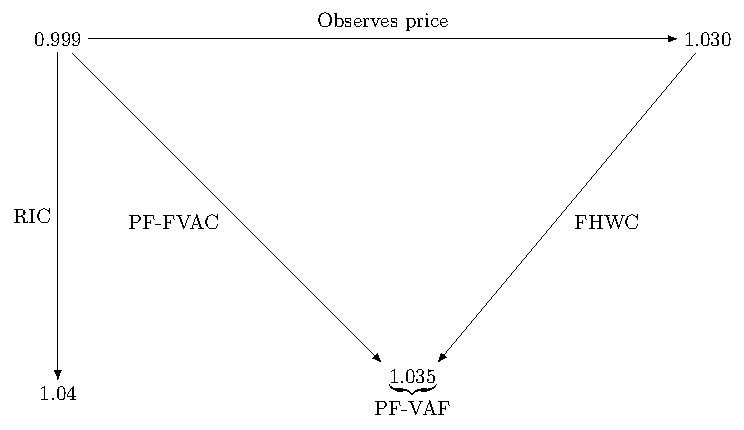
\includegraphics[width=3.5in]{\FigDir/StickyPriceLogic}
  }
  \caption{PF Unconstrained Model: Relation of \GICRaw, \FHWC, \RIC, and \PFFVAC} \label{fig:StickyPriceLogic}
  \footnotesize{A first visualization of the model's logic}
\end{figure}
 % Read in the tex to generate the figure

Just a citation test: \cite{DostenTest}
\cite{friedmanATheory}




% %The paper's results are all easily reproducible \href{https://econ-ark.org/_materials/BufferStockTheory?launch}{interactively on the web} or \href{https://github.com/econ-ark/BufferStockTheory}{on any standard computer system}.  Such reproducibility reflects the paper's use of the open-source \href{https://econ-ark.org}{Econ-ARK} toolkit, which is used to generate all of the quantitative results of the paper, and which integrally incorporates all of the analytical insights of the paper.

% % The Dummy equation below sems to be needed to get the equation numbering in the appendix
% % reliably to start at the next number after the last actual equation number used in the paper

% \clearpage\vfill\eject
% \begin{equation*}
%   \label{eq:Dummy}
% \end{equation*}

% \onlyinsubfile{\bibliography{
%     \texname, % subfile inherits texname from preamble of parent
%     \econtexBib % Default bib database is in Resources/LaTeXInputs
%   }}

\onlyinsubfile{% Allows two (optional) supplements to hard-wired \texname.bib bibfile:
% economics.bib is a default bibfile that supplies anything missing elsewhere
% Add-Refs.bib is an override bibfile that supplants anything in \texfile.bib or economics.bib
\IfFileExists{\econtexRoot/Add-Refs.bib}{
  % then
  \typeout{References in Add-Refs.bib will take precedence over those elsewhere}
  \setboolean{AddRefsExists}{true}
  \setboolean{NeitherExists}{false} % Default is true
}{
  % else
  \setboolean{AddRefsExists}{false} % No added refs exist so defaults will be used
  \setboolean{BothExist}{false}     % Default is that Add-Refs and economics.bib both exist
}

% Deal with case where economics.bib is found by kpsewhich
\IfFileExists{/usr/local/texlive/texmf-local/bibtex/bib/economics.bib}{
  % then
  \typeout{References in default global economics.bib will be used for items not found elsewhere}
  \setboolean{economicsExists}{true}
  \setboolean{NeitherExists}{false}
}{
  % else
  \typeout{Found no global database file}
  \setboolean{economicsExists}{false}
  \setboolean{BothExist}{false}
}

\ifthenelse{\boolean{BothExist}}{
  % then use both
  \typeout{bibliography{\econtexRoot/Add-Refs,\econtexRoot/\texname,economics}}
  \bibliography{\econtexRoot/Add-Refs,\econtexRoot/\texname,economics}
  % else both do not exist
}{ % maybe neither does?
  \ifthenelse{\boolean{NeitherExists}}{
    \typeout{bibliography{\texname}}
    \bibliography{\texname}}{
    % no -- at least one exists
    \ifthenelse{\boolean{AddRefsExists}}{
      \typeout{bibliography{\econtexRoot/Add-Refs,\econtexRoot/\texname}}
      \bibliography{\econtexRoot/Add-Refs,\econtexRoot/\texname}}{
      \typeout{bibliography{\econtexRoot/\texname,economics}}
      \bibliography{         \econtexRoot/\texname,economics}}
  } % end of picking the one that exists
} % end of testing whether neither exists
}
%\bibliography{economics}
\end{document}
\endinput

% If you are editing in Emacs-AucTeX, modify the lines below for your system (otherwise ignore)
% Local Variables:
% eval: (setq TeX-command-list  (assq-delete-all (car (assoc "BibTeX" TeX-command-list)) TeX-command-list))
% eval: (setq TeX-command-list  (assq-delete-all (car (assoc "BibTeX" TeX-command-list)) TeX-command-list))
% eval: (setq TeX-command-list  (assq-delete-all (car (assoc "BibTeX" TeX-command-list)) TeX-command-list))
% eval: (setq TeX-command-list  (assq-delete-all (car (assoc "Biber"  TeX-command-list)) TeX-command-list))
% eval: (add-to-list 'TeX-command-list '("BibTeX" "bibtex LaTeX/%s" TeX-run-BibTeX nil t                                                                              :help "Run BibTeX") t)
% eval: (add-to-list 'TeX-command-list '("BibTeX" "bibtex LaTeX/%s" TeX-run-BibTeX nil (plain-tex-mode latex-mode doctex-mode ams-tex-mode texinfo-mode context-mode) :help "Run BibTeX") t)
% TeX-PDF-mode: t
% TeX-file-line-error: t
% TeX-debug-warnings: t
% LaTeX-command-style: (("" "%(PDF)%(latex) %(file-line-error) %(extraopts) -output-directory=LaTeX %S%(PDFout)"))
% TeX-source-correlate-mode: t
% TeX-parse-self: t
% eval: (cond ((string-equal system-type "darwin")    (progn (setq TeX-view-program-list '(("Skim" "/Applications/Skim.app/Contents/SharedSupport/displayline -b %n LaTeX/%o %b"))))))
% eval: (cond ((string-equal system-type "gnu/linux") (progn (setq TeX-view-program-list '(("Evince" "evince --page-index=%(outpage) LaTeX/%o"))))))
% eval: (cond ((string-equal system-type "gnu/linux") (progn (setq TeX-view-program-selection '((output-pdf "Evince"))))))
% TeX-parse-all-errors: t
% End:
